\documentclass{article}
% Include Package for Image Inclusion & define image types
\usepackage{graphicx}
\DeclareGraphicsExtensions{.pdf,.png,.jpg,.jpeg}

%Title Page
\title{\bf{ENEL 441 Lab Demo \#1}}
\author{Group: GC7}
\date{November 1, 2012}

\begin{document}
\pagestyle{empty}

\maketitle

\pagebreak

%%% MODEL ANALYSIS

\section*{System Model Analysis}
{
\noindent The initial model for the system is given as:

\[ mc\ddot{\theta}(t) = -bc\dot{\theta}(t) + K_mu(t) - Mg \]
\[ \ddot{\theta}(t) = \frac{1}{mc}[K_mu(t) - bc\dot{\theta}(t) -Mg] \]
\\
We can state some substitutions for simplification:

\[ x(t) = c\theta(t) \]
\[ v(t) = c\dot\theta(t) = \dot x(t) \]
\[ a(t) = \dot v(t) = c\ddot\theta(t) = \ddot x(t) \]
\\
so we can rewrite (2) in two different ways:

\[ \dot v(t) = \frac{1}{m}[K_mu(t) - bv(t) - Mg] \]
\[ \ddot x(t) = \frac{1}{m}[K_mu(t) -b\dot x(t) - Mg] \]
\\
Now we can focus on simplifying this even more by looking at our control signal and imaging it has DC (Steady-State) and AC (Transient) parts:

\[ u(t) = C_u + \mu(t) \]
\\
We can set the DC portion equal to the value necessary to cancel out the force of the attached weight:

\[ K_mC_u = Mg \]
\\
Since these cancel, this now gives the system as:

\[ \dot v = \frac{1}{m}[K_m\mu(t) - bv(t)] \]
\[ \ddot x = \frac{1}{m}[K_m\mu(t) - b\dot x(t)] \]

This can be converted via the Laplace Transform to:

\[ sV(s) = \frac{1}{m}[K_m\mu(s) - bV(s)] \]
\[ s^2X(s) = \frac{1}{m}[K_m\mu(s) - bsX(s)] \]

To find the Transfer function for the motor for Velocity and Position Respectively:

\[ V(s)[s + \frac{b}{m}] = \frac{K_m}{m}\mu(s) 
\indent\indent\rightarrow\indent\indent
H(s) = \frac{V(s)}{\mu(s)} = \frac{K_m}{ms + b} \]
\\
\[ X(s)[ms^2 +bs] = K_m\mu(s)
\indent\indent\rightarrow\indent\indent
G(s) = \frac{X(s)}{\mu(s)} = \frac{K_m}{s(ms + b)} \]
\\
However, we also need the controller (ie. compensator) for our system such that our car will be as efficient as possible:

\[ C(s) = \frac{\mu(s)}{E(s)} = ? \]

Where $E(s)$ is the Laplace Transform of the positional error $e(t)$:

\[ e(t) = X_{des} - x(t) \]
\[ E(s) = \frac{X_{des}}{s} - X(s) \]
\\
We must find the compensator transfer function. It must be a PID controller (Type-2 System Controller) as it is required to bring both the error in position and speed down to zero. The control signal function will result as: 

\[\mu = K_pe(t) + K_i \int e(t) + K_d\frac{de(t)}{dt}\]

Via Laplace Transform:
\[\mu (s) = K_pE(s) + K_i \frac{E(s)}{s} + K_dsE(s)\]

Which gives us:
\[C(s) = \frac{\mu (s)}{E(s)} = K_P + \frac{K_i}{s} + K_ds\]
\\
}

\pagebreak 

\section*{Simulink Models}
{
\begin{figure}[h]
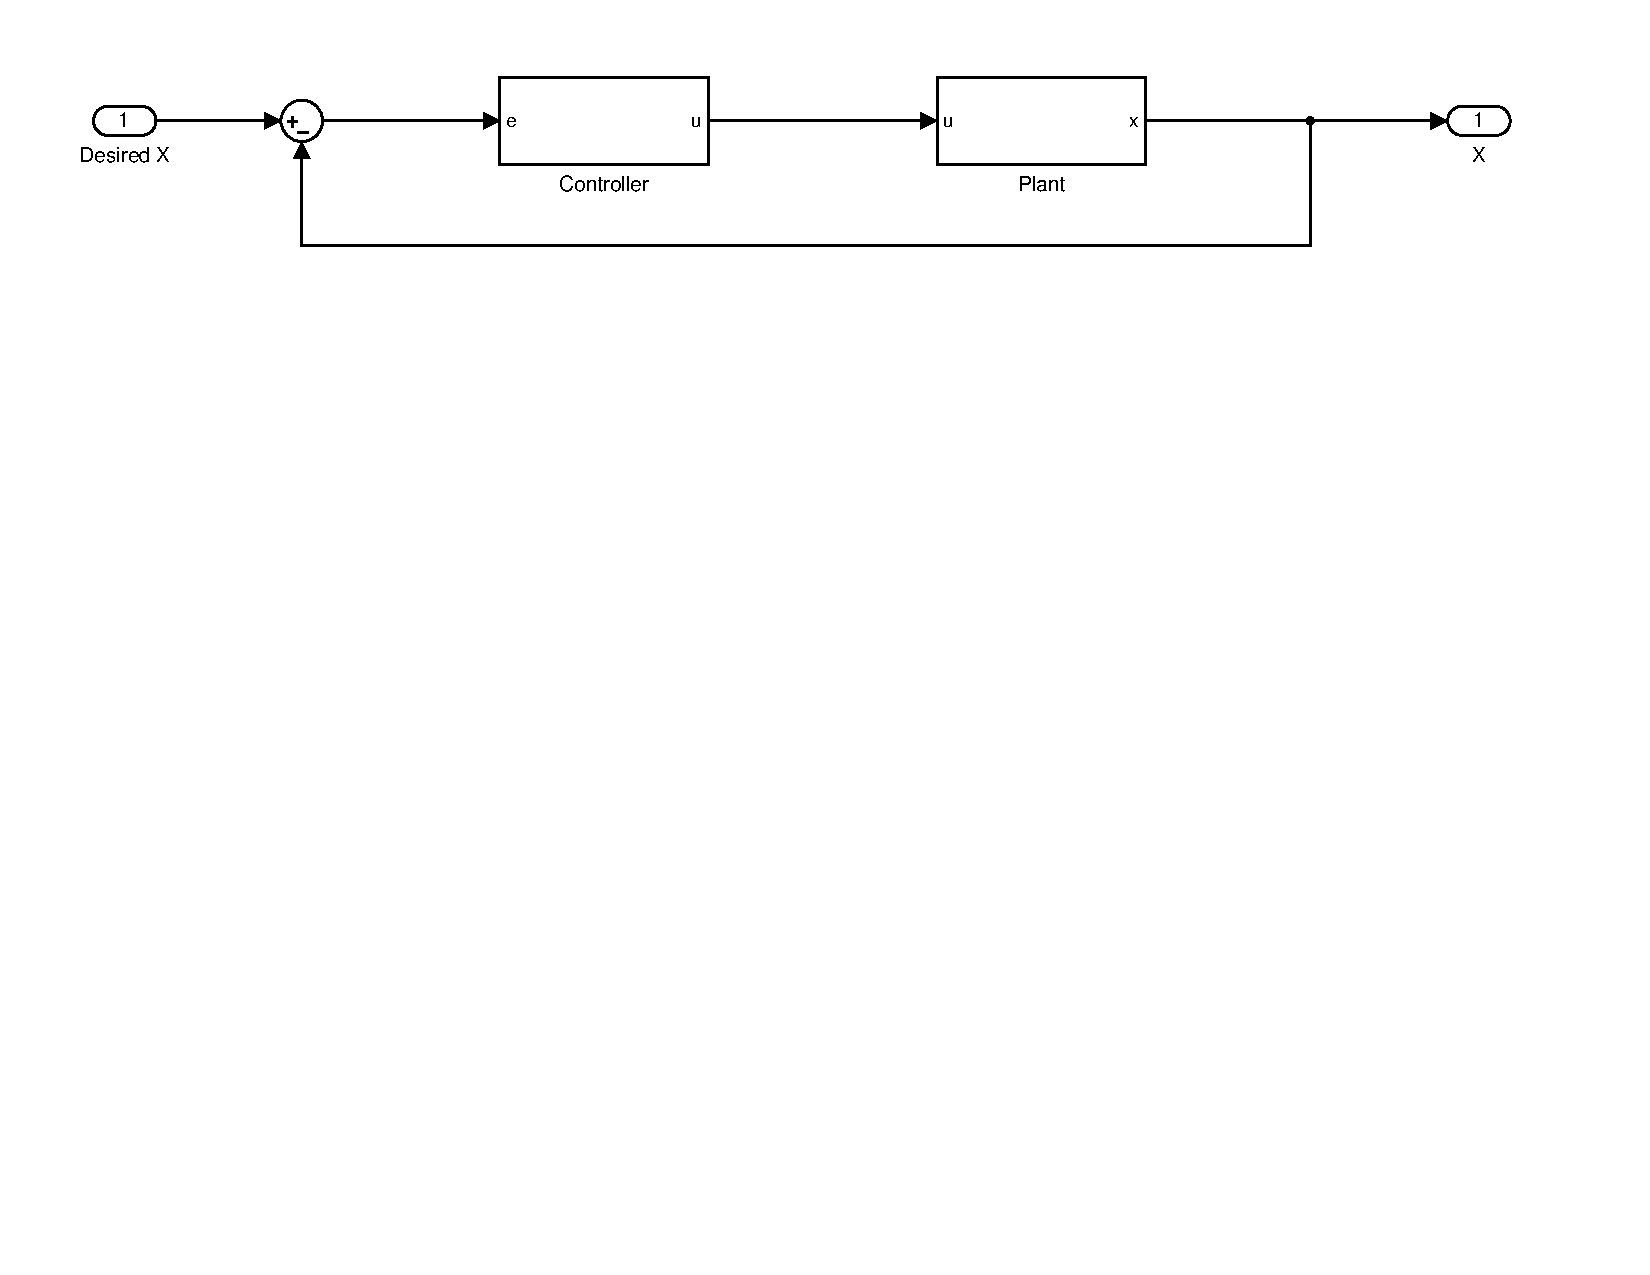
\includegraphics[width=14cm]{PlantModel.pdf}
\caption{Simple Controller-Plant Model}
\end{figure}

\pagebreak

\begin{figure}[h]
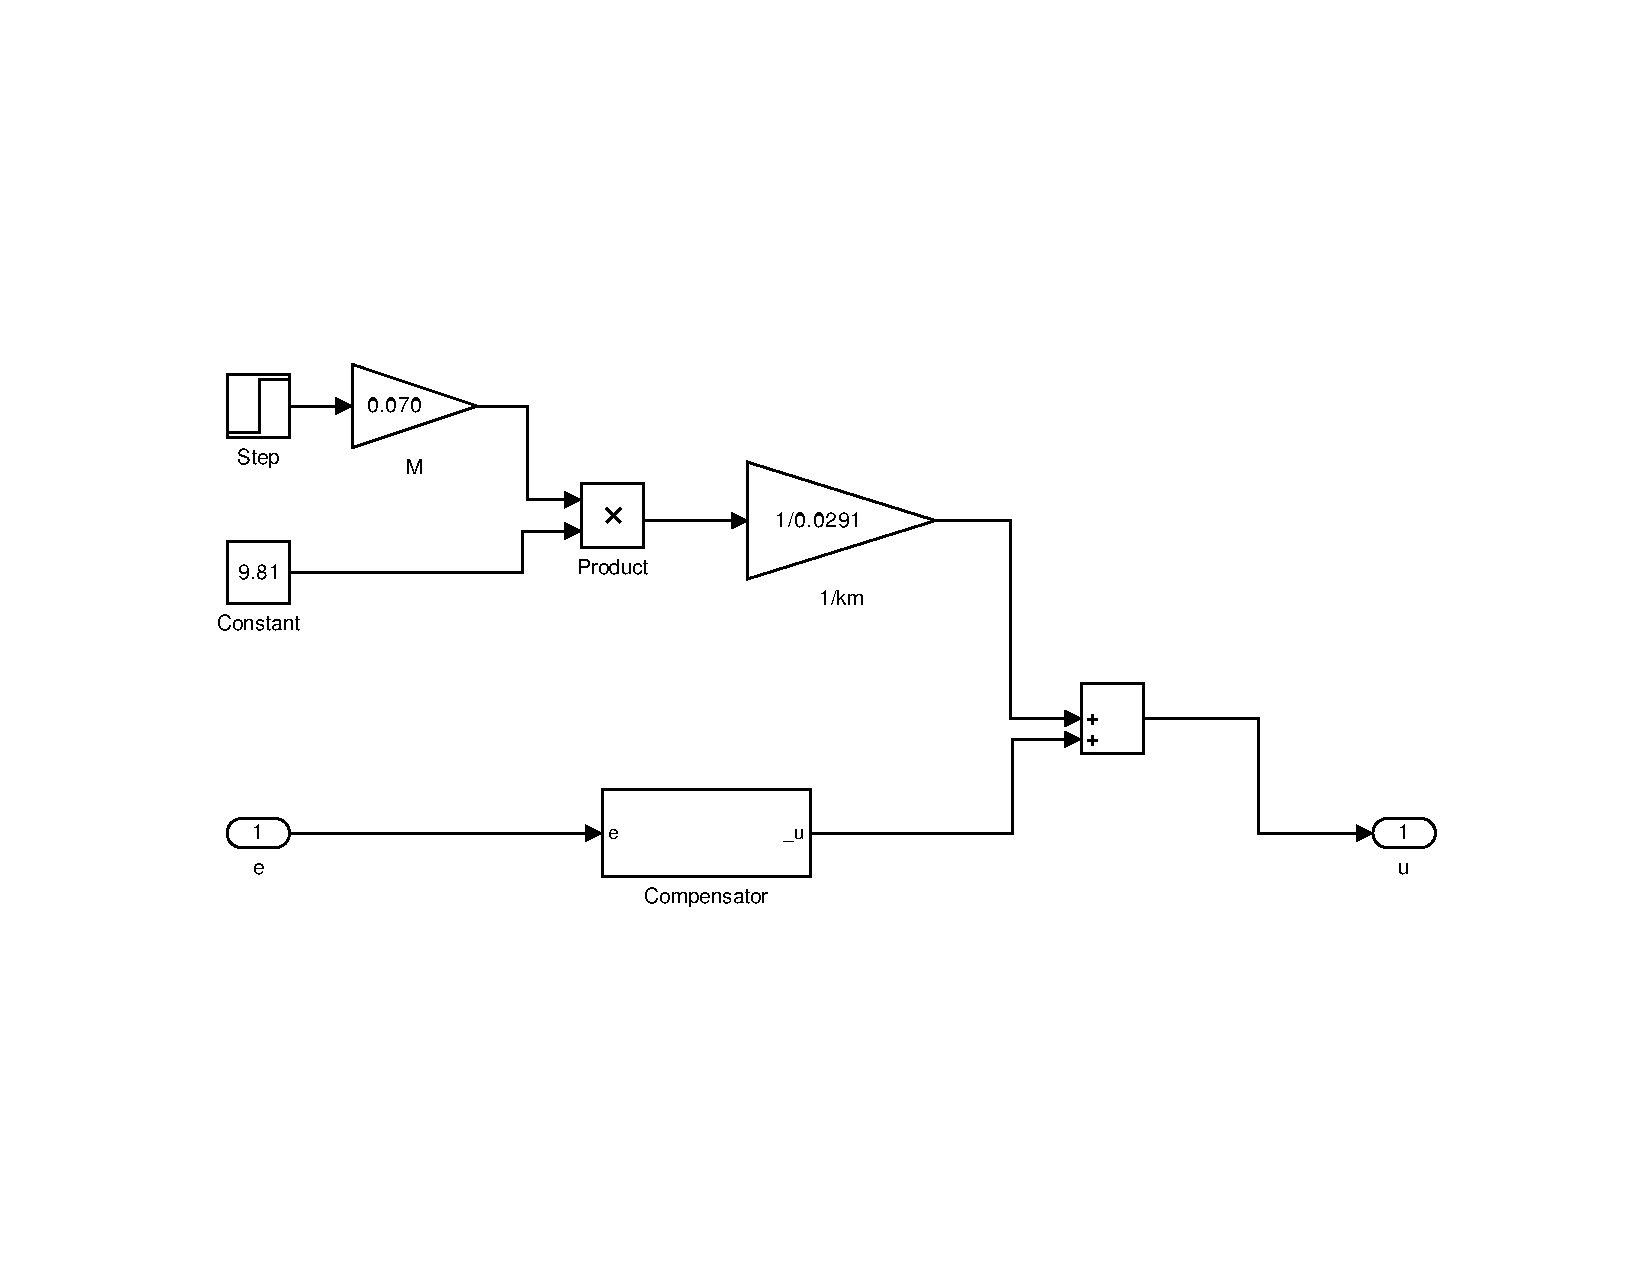
\includegraphics[width=14cm]{ControllerModel.pdf}
\caption{Controller Subsystem Model}
\end{figure}

\pagebreak

\begin{figure}[h]
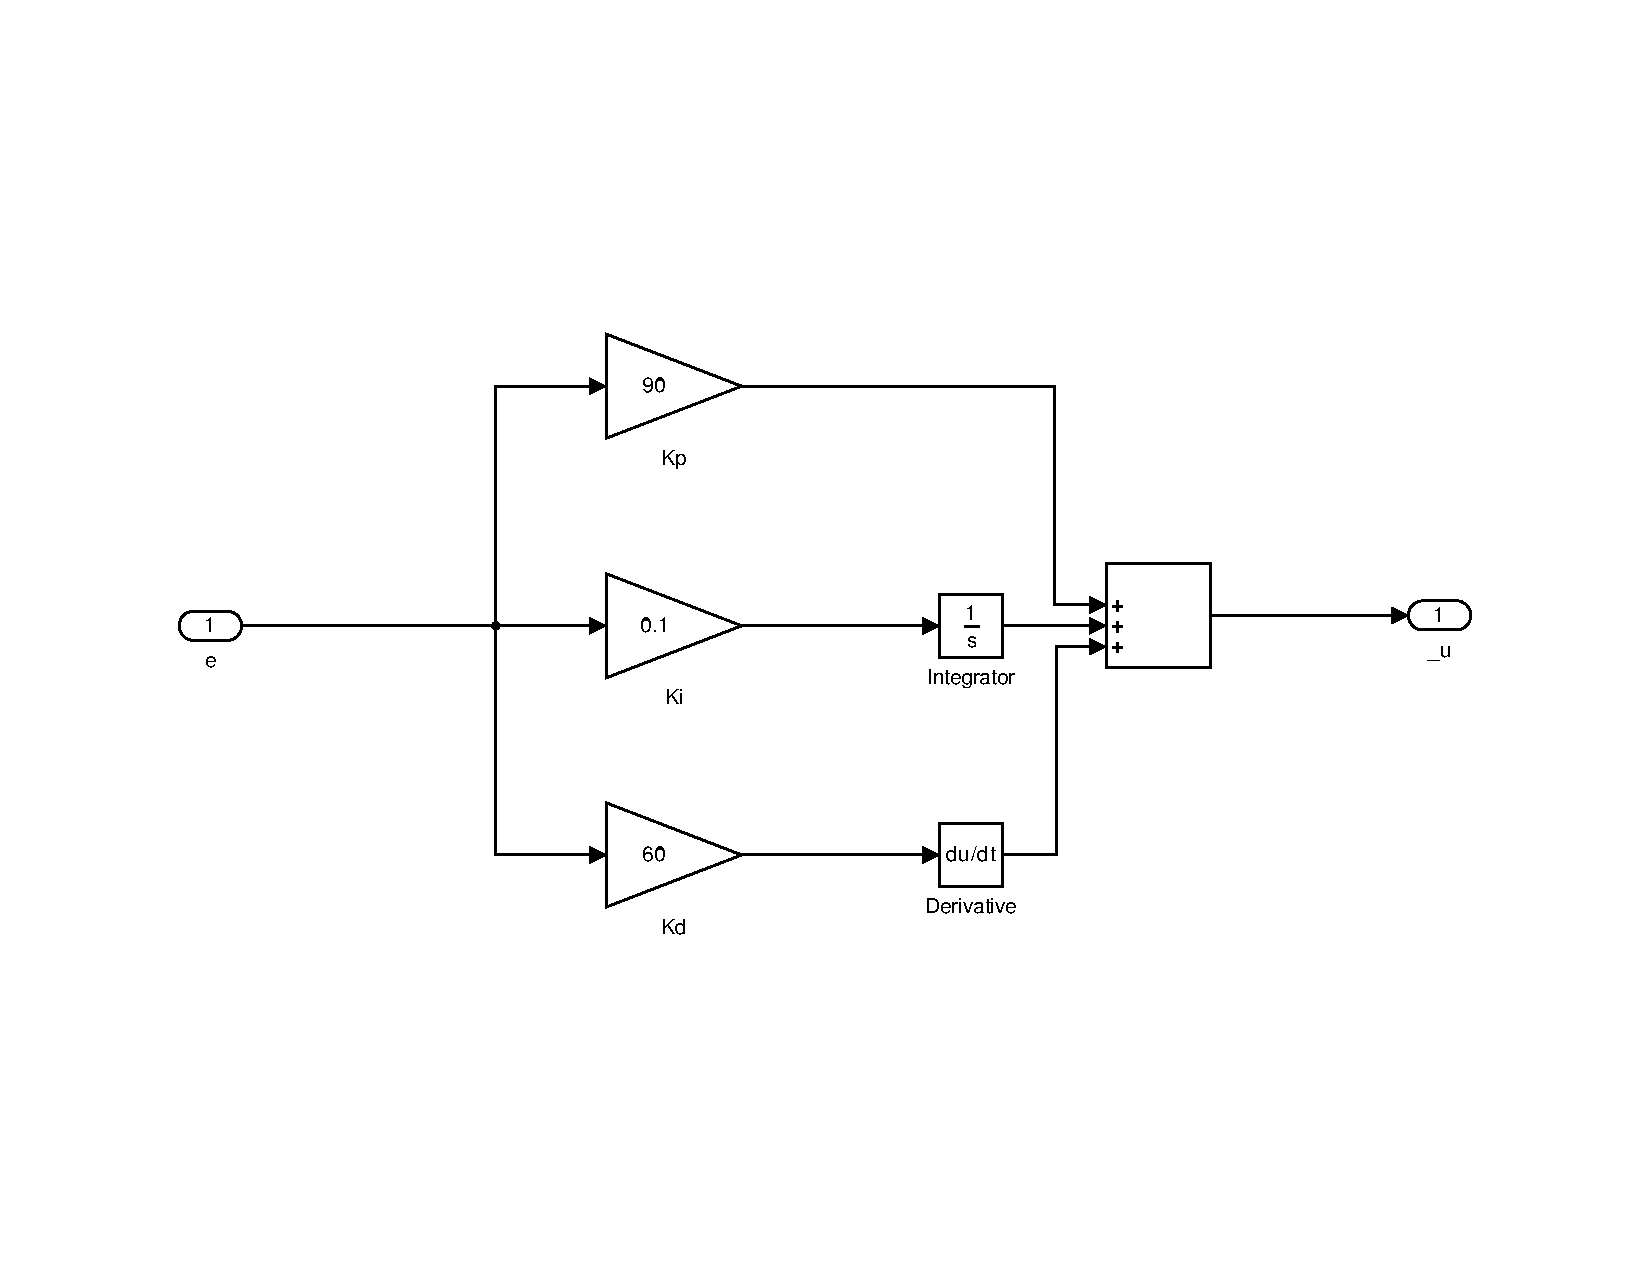
\includegraphics[width=14cm]{Compensator.pdf}
\caption{Compensator Subsystem Model, Transfer Function C(s)}
\end{figure}

\pagebreak

\begin{figure}[h]
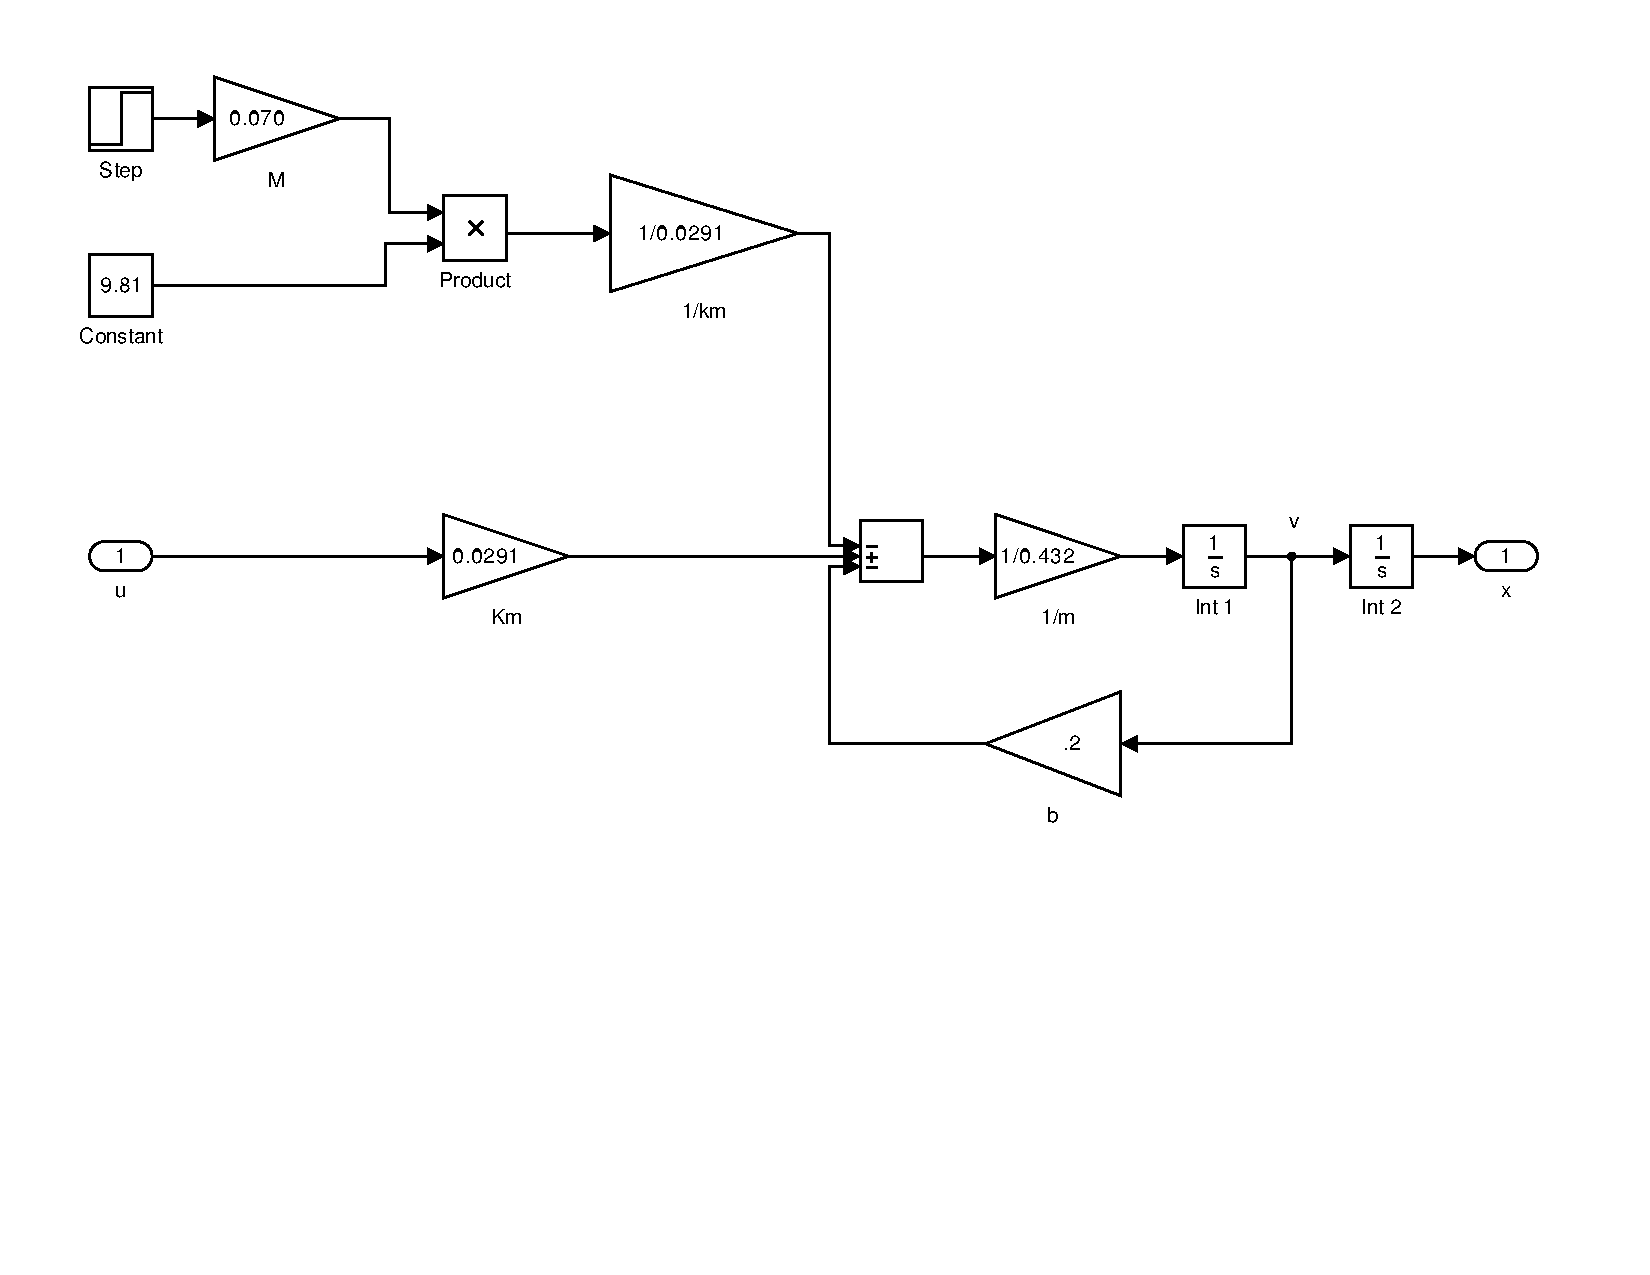
\includegraphics[width=14cm]{PlantSystem.pdf}
\caption{Plant Subsystem Model, Transfer Function G(s)}
\end{figure}

\pagebreak

\begin{figure}[h]
\setcounter{page}{8}
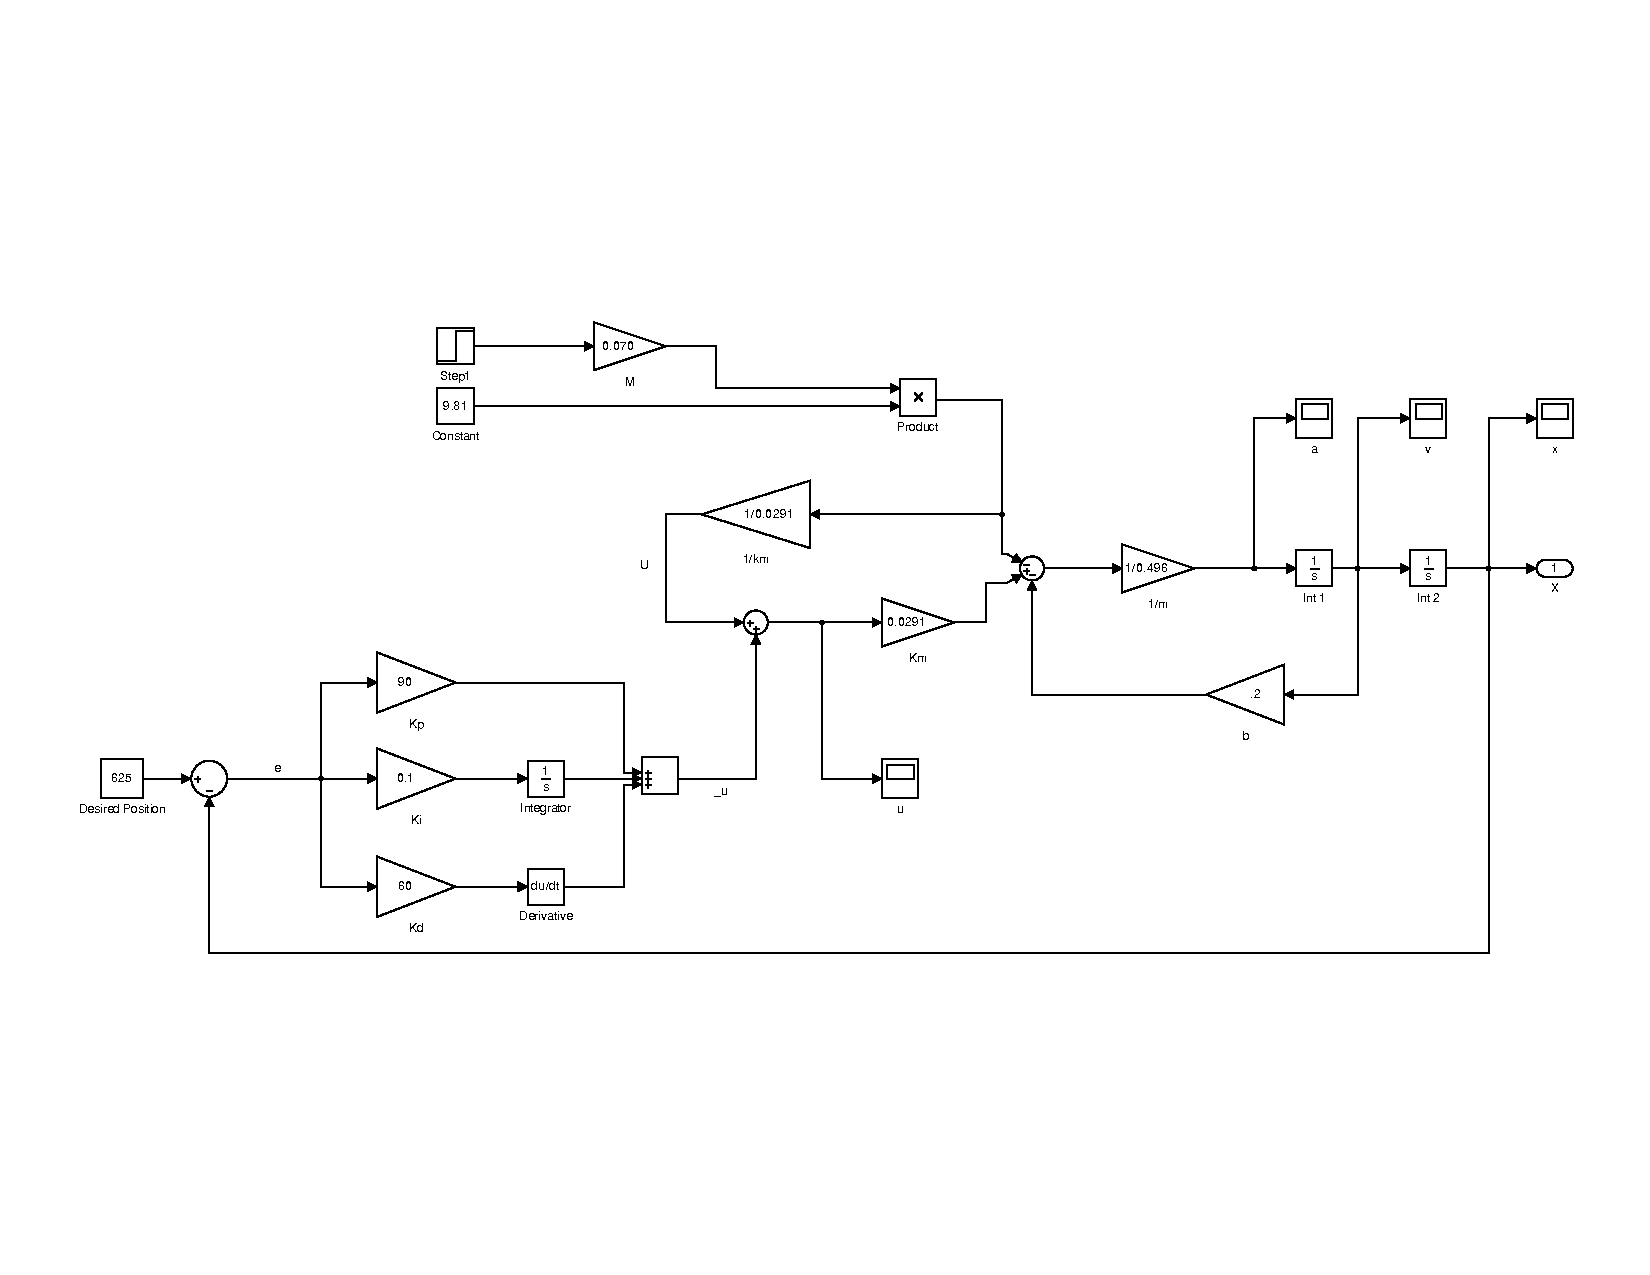
\includegraphics[height = 19cm]{DemoModelPID.pdf}
\caption{Fully expanded System Model}
\end{figure}
\pagebreak
}

\section*{Observational Data}
{
The value of the Motor Constant $K_m$ was found by changing the attached weight's mass, and then finding the highest speed at which the car wouldn't move. The following graph is the linearized plot of the recorded data:
\\
\\
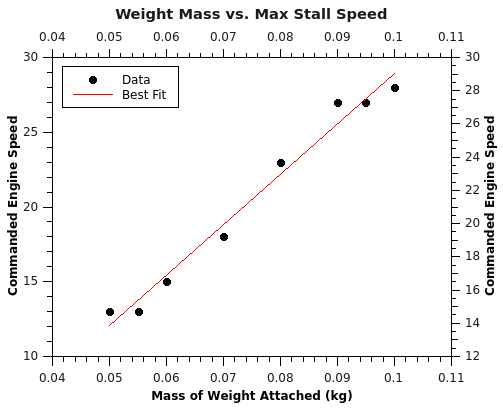
\includegraphics[width=14cm]{MotorConstantGraph.png}
\\
\\
From the graph and the relationship with the motor constant, we can calculate it to be:
\\
\\
\[ K_m = \frac{\Delta M g}{\Delta C_u} = 0.0291 \]

\pagebreak

In order to find the value of the coefficient of friction, $b$, we can compare the simulated system to that of the actual car for different values of $b$. The following graph showcases the effect that different values have on the system along with the recorded observed system response:
\\
\\
\center{
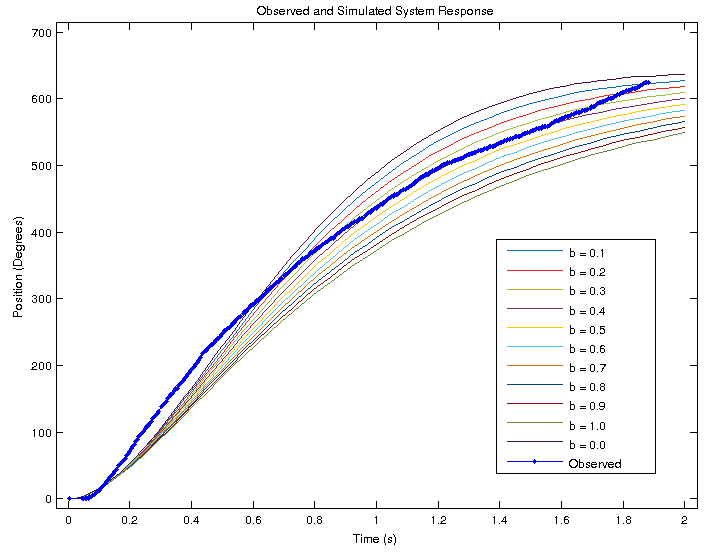
\includegraphics[width=14cm]{ComparitiveAnalysis.png}
}
}
\\
\\
If we compare the actual response to that of the simulation, we see that the closest value of $b$ which approximates the system is:
\\
\[ b = 0.4 \]
\\
\pagebreak
\\
If we isolate the simulation with our chosen value of $b$ and plot it against our output we get:
\\
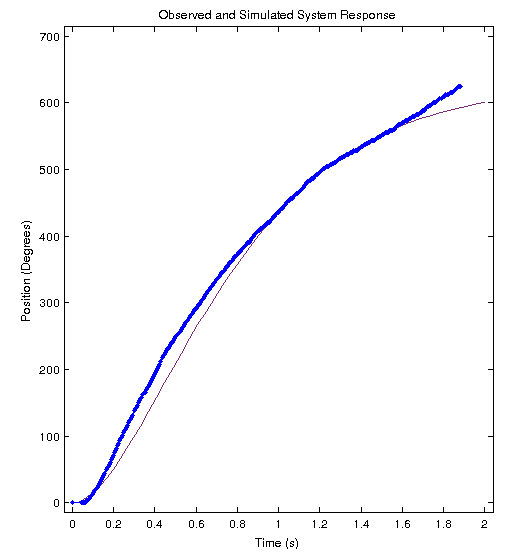
\includegraphics[width=14cm]{ChosenSimComparitive.png}
\end{document}